\section{Methoden}

\subsection{Allgemeine Funktionsweise eines Spektrographen}
Mit Hilfe eines Spektrographen kann man Licht in seine Farben zerlegen. Dabei besteht ein Spektrograph im Wesentlichen aus folgenen Komponenten:

\begin{itemize}

\item Teleskop: Das Teleskop wird benötigt, um Licht zu sammeln und es zu fokussieren.

\item Spalt: Der Spalt schirmt unerwünschte Störquellen ab und sorgt dafür, dass am Dispersionelement ankommende Strahlung im besten Fall von einem Punkt ausgeht, da sich sonst die Auflösung verringert. Dabei kann die Spaltbreite allerdings nicht belibig klein gewählt  werden, da dadurch natürlich auch die Intensität des Lichts abnimmt. Deshalb muss hier ein Optimum gefunden werden.

\item Kollimator: Der Kollimator erzeugt aus dem einfallenden Licht paralleles Licht.

\item Dispersionselement: Das Dispersionselement ist der Hauptbestandteil des Spektrographen. Es trennt das Licht in Abhängigkeit von der Frequenz. Dabei kann es ein Prisma, oder auch ein Gitter sein. (Das Prisma trennt das Licht auf Grund der Frequenzabhängigkeit der Brechung, während die Trennung beim Gitter durch Interferenzeffekte hervorgerufen wird.)

\item Kamera-Objektiv: Das Kamera-Objektiv wird benötigt, um das durch das Dispersionselement erzeugte Spektrum auf den CCD-Detektor abbzubilden.

\item CCD-Detektor: Der CCD-Detektor digitalisiert schließlich das Bild des Spektrums.

\end{itemize}

Im Bamberger Spektrographen wird ein Blaze-Reflektionsgitter verwendet. (siehe Abb. \ref{fig:101} und \ref{fig:102} ) Dieses hat regelmäßig angeordnete geneigte Furchen und bietet so den Vorteil, dass das Intensitätsmaximum in Richtung des dispergierten Lichtes verschoben wird. 

\begin{figure}
		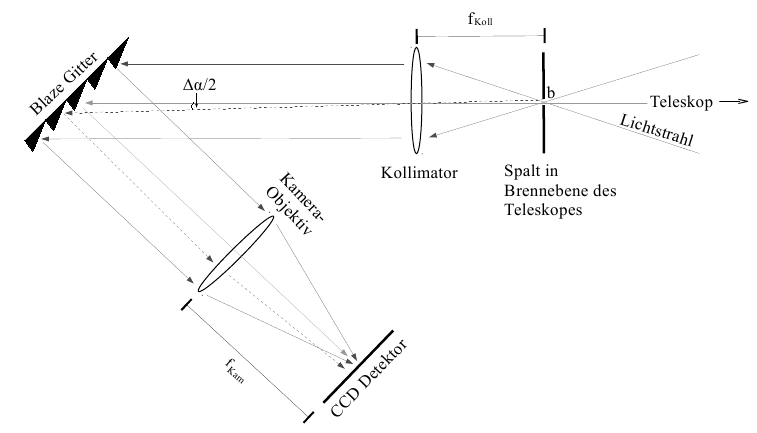
\includegraphics[width=.9\textwidth]{images/Abbildung101}
\caption{ Schematischer Aufbau eines Gitterspektrographen mit Blaze-Gitter }
\label{fig:101}
\end{figure}

\begin{figure}
        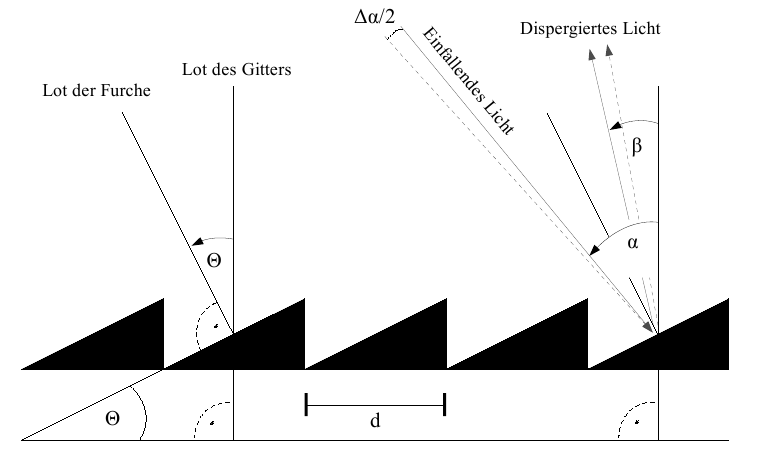
\includegraphics[width=.9\textwidth]{images/Abbildung102.png}
\caption{ Beispiel eines Blaze-Gitters und seiner charakteristischen Größen }
\label{fig:102}
\end{figure}

\begin{figure}
        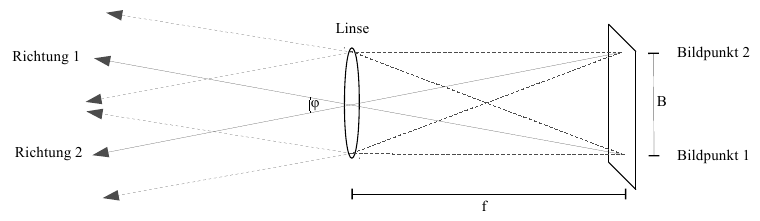
\includegraphics[width=.9\textwidth]{images/Abbildung103.png}
\caption{ Abbildungsmaßstab einer Linse }
\label{fig:103}
\end{figure}


\subsection{Funktionsweise eines Echelle-Spektrographen}
c

\subsection{Auflösungszeugs/Vorübungen}
aus Vorübungen einbringen!

\subsection{Durchführung der Messung}
e

\subsection{Datenreduktion}
f

\subsection{Auswertung}
g

